\documentclass[a4paper]{report} % Formato plantilla

\usepackage{graphicx}
\usepackage[utf8]{inputenc} % Para poder usar caracteres especiales
\usepackage[spanish]{babel} % Para poder usar caracteres especiales

\begin{document} % Inicio del documento Template
  \begin{titlepage}
    \centering
    {\scshape\LARGE Universidad Católica de Pereira\par}
    \vfill
    {\scshape\LARGE Electiva IV Power BI\par}
    \vfill
    {\huge\bfseries Parcial Power Bi\par}
    \vfill
    {\Large\itshape Juan David Garcia Acevedo\par}
    \vfill
    Docente de la materia\par
	   Carlos Andres \textsc{Cortes}
    \vfill
    {\Large\today\par}
  \end{titlepage}
%======================================================================
  \tableofcontents % Para crear los índices
    \part{Parcial de Power Bi}
      \chapter{Obesity Data Set - Punto 1}
        \section{Distribución del peso total por rango de edad y género} 
            \paragraph{}\mbox{} \\
            El data set trabajado con Power Bi es sobre la obesidad, al abrir el data set he decidido cambiar los valores de la columna Height de número decimal, a número decimal fijo así se ve mejor representada.\\

              \begin{figure}[htb]
                \centering
                  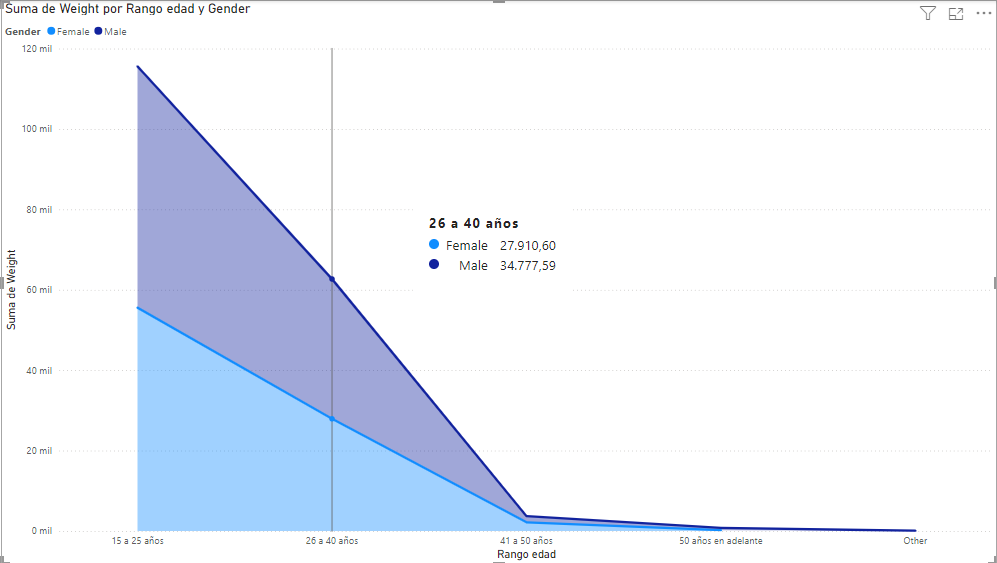
\includegraphics[width=\textwidth]{Images/pesoporgenero.png}
                  \caption{Grafica de \textbf{Peso por Genero}.}
              \end{figure}
Se hace una distribución del peso total por rango de edad y género, donde se ve la distribución del peso total por diferentes rangos de edad, diferenciada por género. Los hombres y las mujeres alcanzan su mayor peso entre los 26 y 40 años, esto sugiere que el grupo tiende a tener un peso corporal promedio más elevado.\\A partir de los 40 años, el peso dismiyune, probablemente debido a cambios en el cuerpo y en el estilo de vida. Además, los hombres presentan un mayor peso total que las mujeres en todos los grupos de edad, aunque esto requiere de una mayor investigación y mayor detalle.
         \section{Peso por altura según rangos de edad}
            \paragraph{}\mbox{} \\
            Grafica de peso por altura según rangos de edad
            \begin{figure}[htb]
                \centering
                  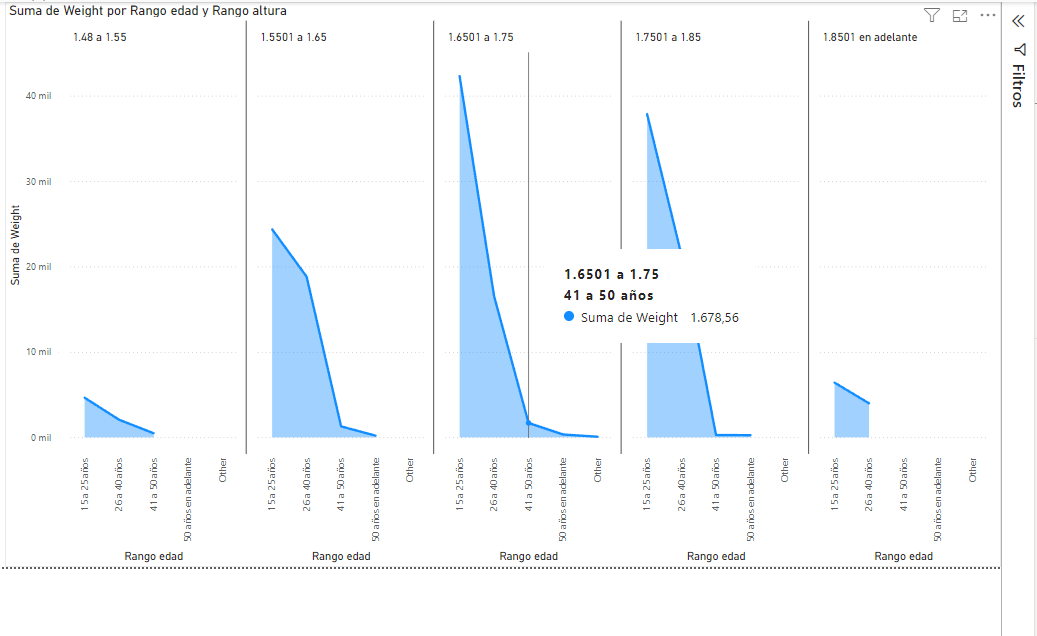
\includegraphics[width=\textwidth]{Images/pesoporaltura.png}
                  \caption{Grafica de \textbf{Peso por altura}.}
              \end{figure}

La gráfica muestra la relación entre el peso y la altura en distintos grupos de edad. En todos los grupos se puede ver un incremento en el peso a medida que la altura aumenta, puede ser por la masa corporal y la altura, las personas de 15 a 25 años tiene un menor peso comparado con los individuos de 26 a  40 años. Personas con estatura de 1.75 y 1.85 metros son los que tienen mayor peso, mientras que los que miden menos tienden a tener un peso inferior.
            \section{Peso según consumo de alimentos con alto valor calórico}
              \paragraph{}\mbox{} \\

\begin{figure}[htb]
                \centering
                  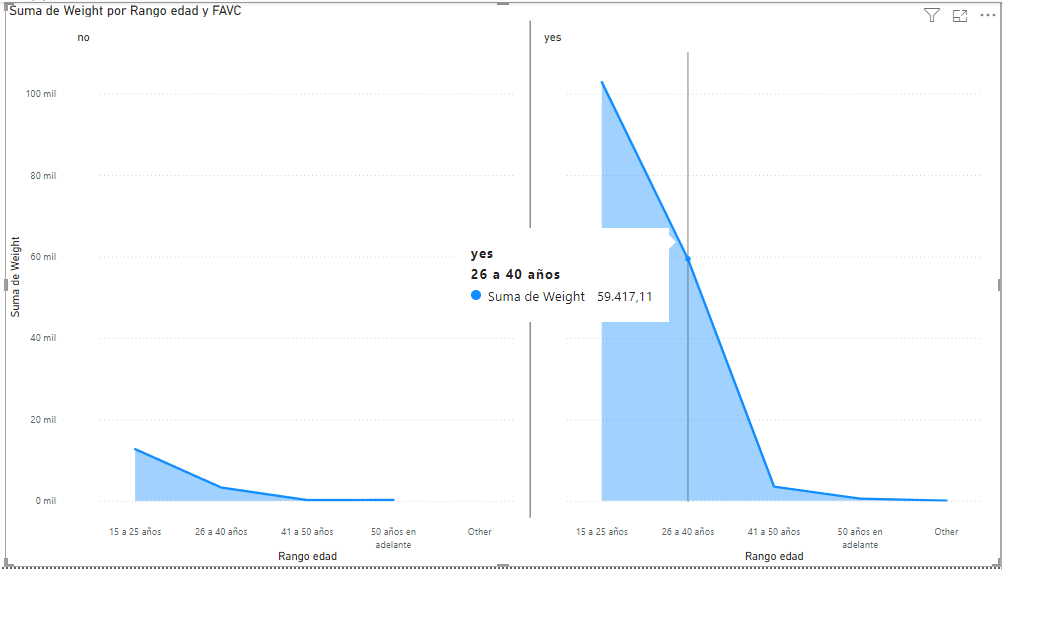
\includegraphics[width=\textwidth]{Images/pesoporalimentoscalorias.png}
                  \caption{Grafica de \textbf{Peso por alimentos altos en calórias}.}
              \end{figure} 

              La grafica muestra la relación entre el peso y el consumo de alimentos de alto valor calórico (FAVC). Aquellos que consumen estos alimentos son los que con mayor frecuencia presentan pesos mayores, entre los 26 y 40 años. Por otro lado, las personas que no consumen alimentos calóricos muestran un menor peso en todos los rangos de edad.
        \section{Peso según consumo de vegetales}
            \paragraph{}\mbox{} \\
              \begin{figure}[htb]
                \centering
                  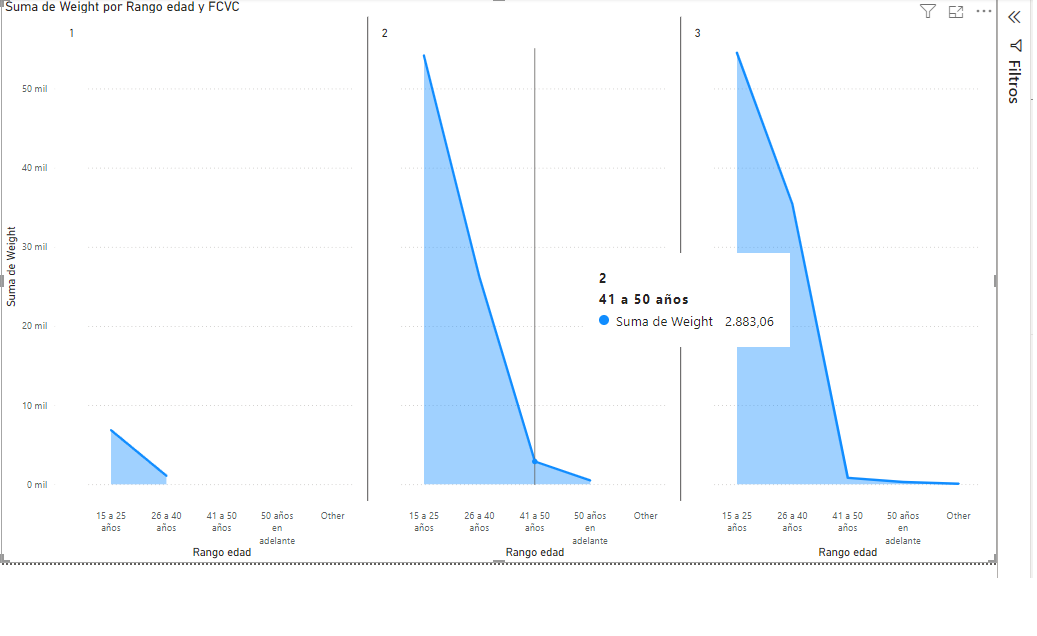
\includegraphics[width=\textwidth]{Images/pesoporalimentosvegetales.png}
                  \caption{Grafica de \textbf{Peso por alimentos vegetales}.}
              \end{figure} \\


El peso total se distribuye en función del consumo de vegetales y los rangos de edad. Existe una relación inversa entre el consumo de vegetales y el peso: aquellos que consumen más vegetales tienden a tener un peso menor, particularmente en el rango de 26 a 40 años. Las personas que consumen menos vegetales muestran un mayor peso en todos los grupos de edad.

        \section{Peso según número de comidas diarias}
            \paragraph{}\mbox{} \\
           Peso según número de comidas diarias
           
La gráfica revela la relación entre el peso y el número de comidas diarias. Los grupos con un número intermedio de comidas (2 o 3) presentan un peso mayor, en especial entre los 26 y 40 años. En cambio, los grupos que hacen menos o más comidas muestran un peso menor, aunque las diferencias no son muy marcadas.

           \section{Peso según consumo de alimentos con alto valor calórico}
              \paragraph{}\mbox{} \\

\begin{figure}[htb]
                \centering
                  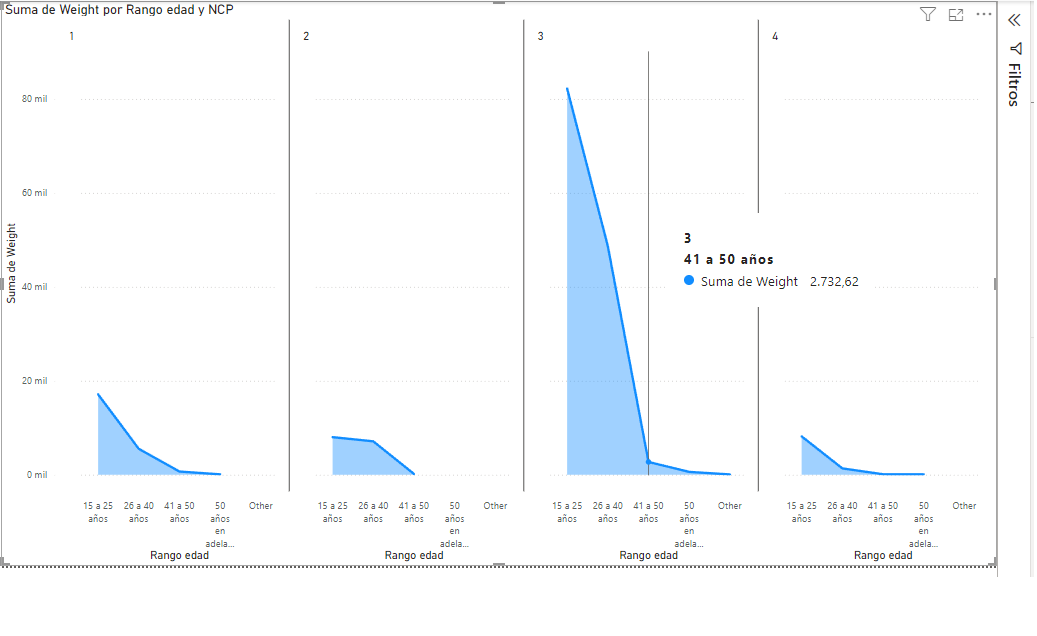
\includegraphics[width=\textwidth]{Images/pesoporcomidasdiarias.png}
                  \caption{Grafica de \textbf{Peso por el número de comidas diarias}.}
              \end{figure} 



\section{Peso según monitoreo de ingesta calórica}
\paragraph{}\mbox{} \\
\begin{figure}[htb]
                \centering
                  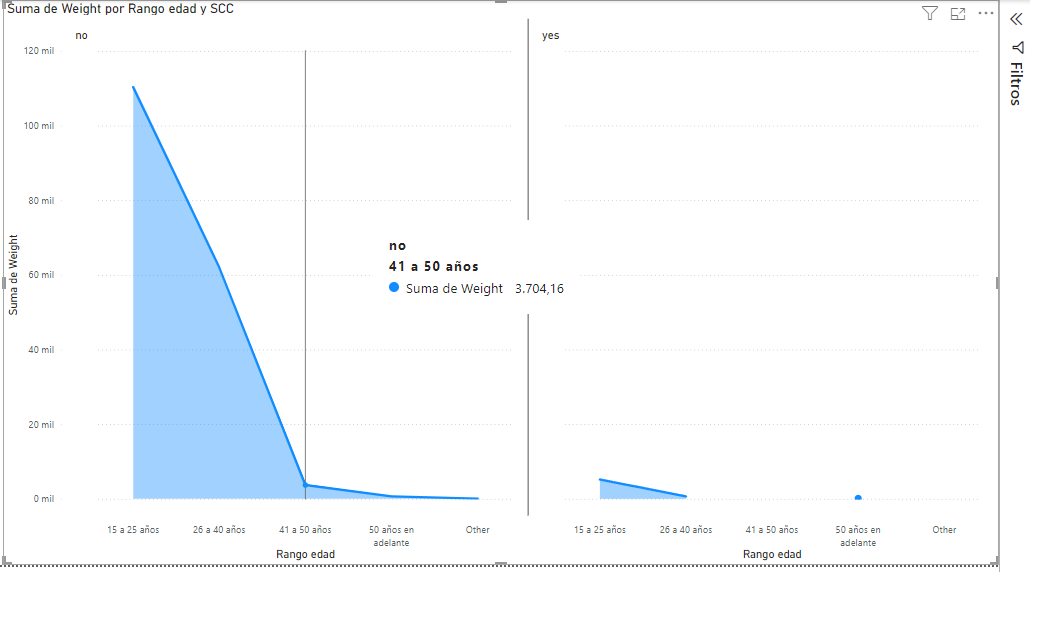
\includegraphics[width=\textwidth]{Images/pesopormonitoreocalorias.png}
                  \caption{Grafica de \textbf{Peso por el monitoreo de calórias}.}
              \end{figure} 
El monitoreo de la ingesta calórica parece influir en el peso. Aquellos que controlan su consumo calórico muestran un peso significativamente menor, sobre todo entre los 26 y 40 años. En contraste, quienes no controlan su ingesta calórica presentan un mayor peso en todos los grupos de edad.
\section{Peso según hábito de fumar}
\paragraph{}\mbox{} \\
\begin{figure}[htb]
                \centering
                  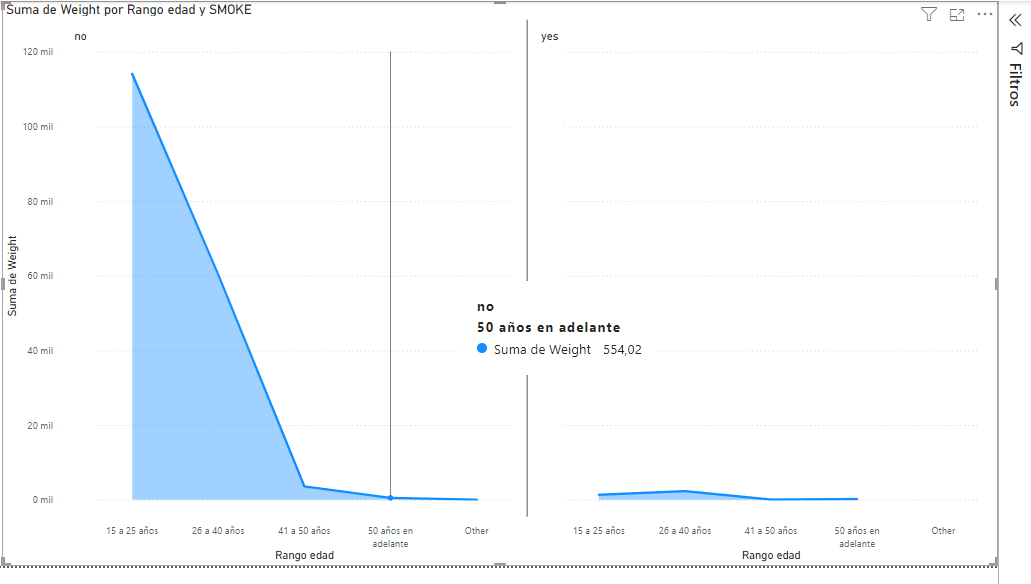
\includegraphics[width=\textwidth]{Images/pesoporfumar.png}
                  \caption{Grafica de \textbf{Peso por fumar}.}
              \end{figure} 
La gráfica muestra la relación entre fumar y el peso. Las personas que no fuman tienden a tener un mayor peso en el rango de 15 a 40 años, mientras que las que fuman presentan un peso significativamente menor. Este patrón es más evidente en los grupos de edad jóvenes, mientras que en personas mayores las diferencias son menos marcadas.
\section{Peso según frecuencia de consumo de agua}
\paragraph{}\mbox{} \\
\begin{figure}[htb]
                \centering
                  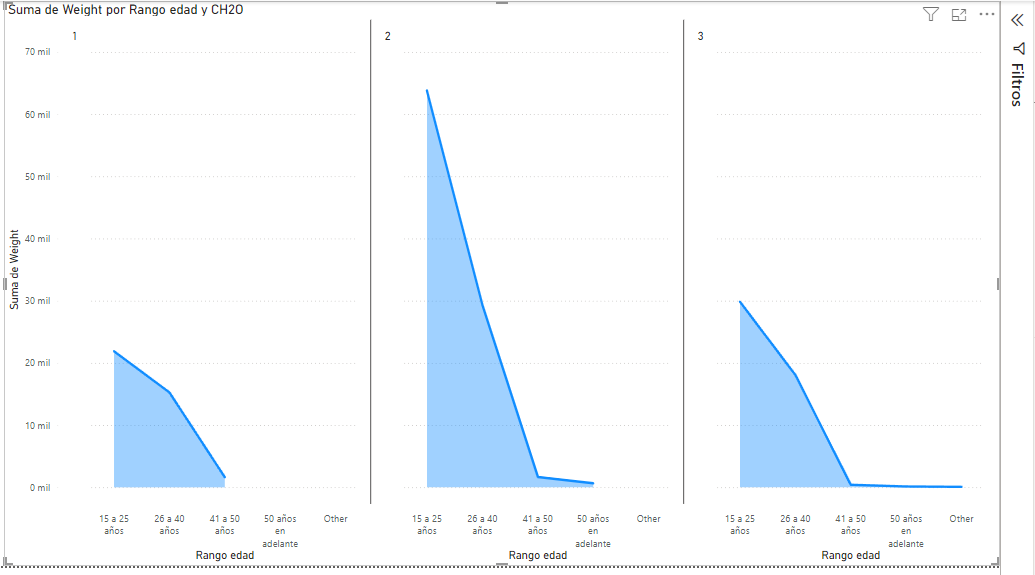
\includegraphics[width=\textwidth]{Images/pesoporagua.png}
                  \caption{Grafica de \textbf{Peso por agua}.}
              \end{figure} 
La frecuencia de consumo de agua también parece afectar el peso. Las personas que consumen una cantidad moderada de agua (grupo 2) muestran el mayor peso, especialmente entre los 26 y 40 años. En cambio, los que beben menos o más agua tienden a tener un peso menor.
\section{Peso según antecedentes familiares de sobrepeso}
\paragraph{}\mbox{} \\
\begin{figure}[htb]
                \centering
                  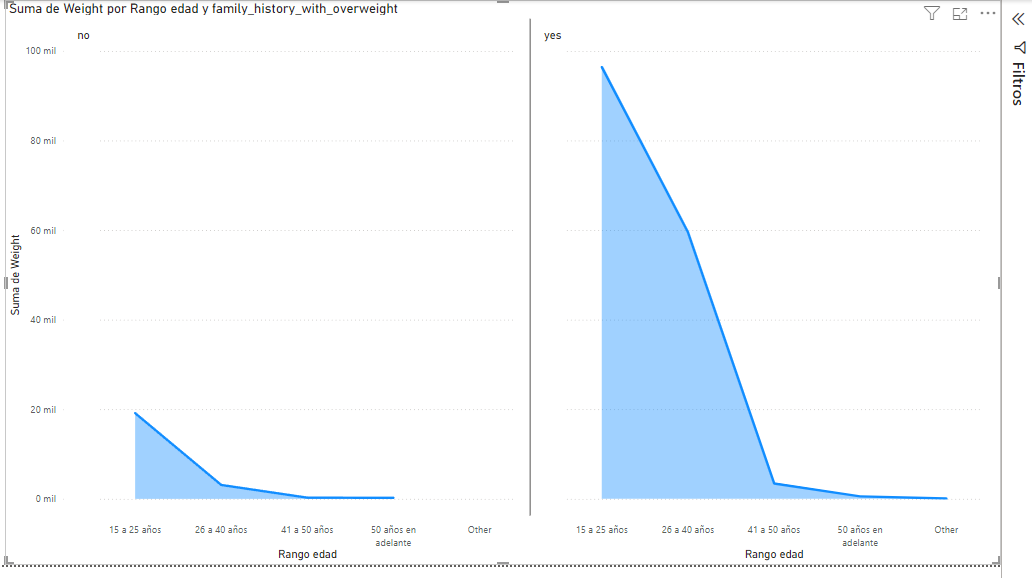
\includegraphics[width=\textwidth]{Images/pesoporhistoriafamiliar.png}
                  \caption{Grafica de \textbf{Peso por el historial familiar}.}
              \end{figure} 
El peso total tiende a ser mayor en aquellos con antecedentes familiares de sobrepeso, sobre todo en el rango de edad de 26 a 40 años. Quienes no tienen antecedentes familiares suelen pesar menos en todos los grupos de edad.
\section{Peso según frecuencia de ejercicio}
\paragraph{}\mbox{} \\
\begin{figure}[htb]
                \centering
                  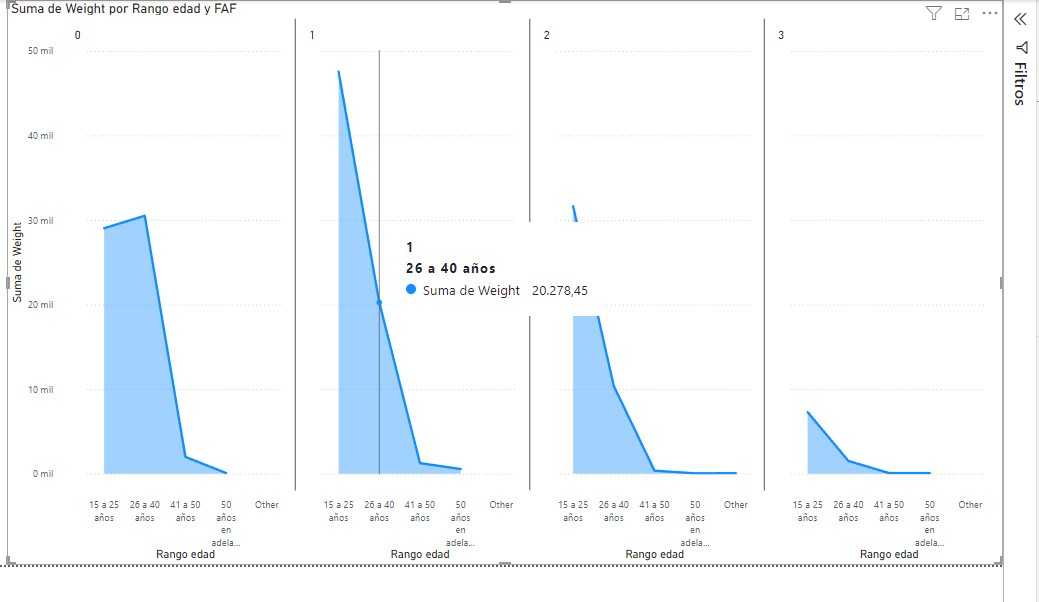
\includegraphics[width=\textwidth]{Images/pesoporejercicio.png}
                  \caption{Grafica de \textbf{Peso por ejercicio}.}
              \end{figure} 
El análisis muestra que el grupo que realiza ejercicio de manera moderada (grupo 2) tiende a tener un peso menor, en especial entre los 26 y 40 años. Los grupos que hacen ejercicio con menor o mayor frecuencia tienen un peso más elevado, aunque las diferencias no son tan consistentes.
\section{Peso según uso de tecnologías}
\paragraph{}\mbox{} \\
\begin{figure}[htb]
                \centering
                  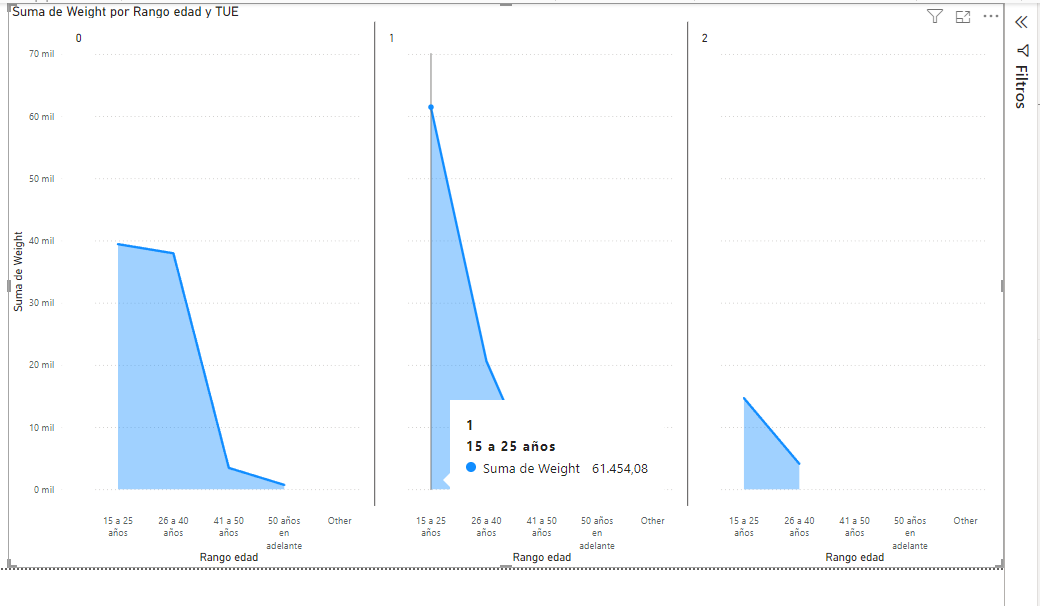
\includegraphics[width=\textwidth]{Images/pesoportecnologias.png}
                  \caption{Grafica de \textbf{Peso por tecnologias}.}
              \end{figure} 
La relación entre el uso de tecnologías y el peso es menos clara. Sin embargo, las personas que utilizan menos tecnología tienden a tener un peso menor, particularmente en el rango de 26 a 40 años. El grupo que usa más tecnología muestra un peso ligeramente mayor en ese rango etario.
\section{Peso según el uso de transporte}
\paragraph{}\mbox{} \\
\begin{figure}[htb]
                \centering
                  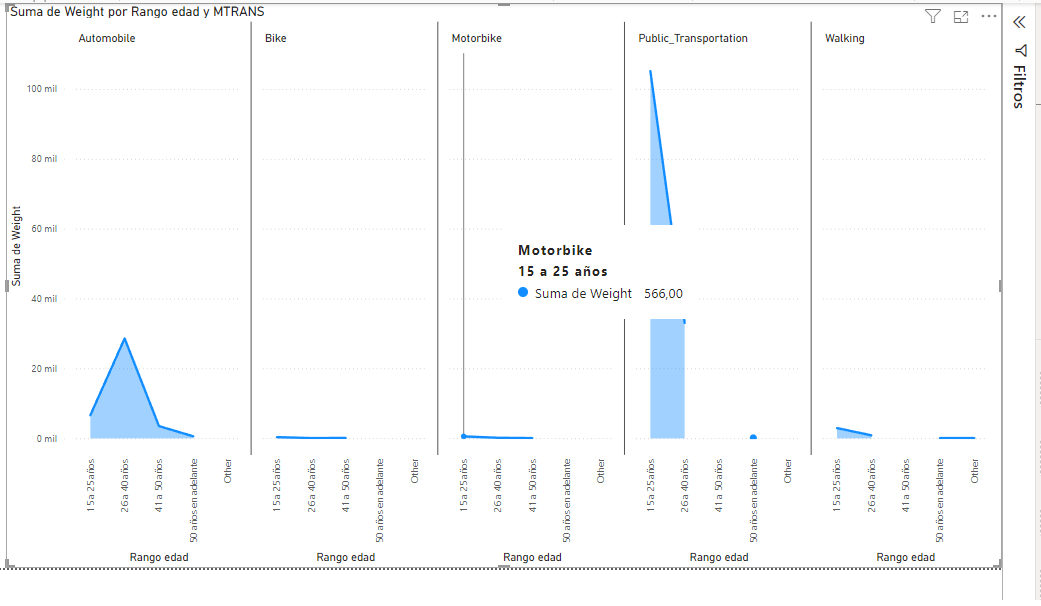
\includegraphics[width=\textwidth]{Images/pesoportransporte.png}
                  \caption{Grafica de \textbf{Peso por transporte}.}
              \end{figure} 
El tipo de transporte utilizado también parece tener un efecto en el peso. Las personas que usan más el automóvil tienden a tener un mayor peso, en especial entre los 26 y 40 años. Por el contrario, aquellos que caminan o usan bicicleta tienden a pesar menos.
\section{Tipo de obesidad según rangos de edad}
\paragraph{}\mbox{} \\
\begin{figure}[htb]
                \centering
                  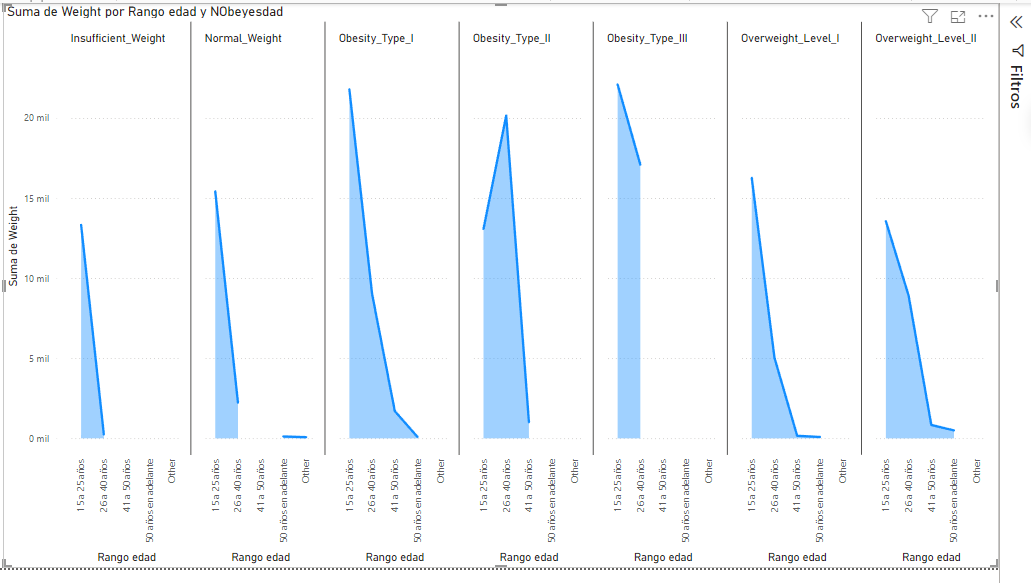
\includegraphics[width=\textwidth]{Images/pesotipoobesidad.png}
                  \caption{Grafica de \textbf{Peso por el tipo de obesidad}.}
              \end{figure} 
La gráfica muestra que en el grupo de 15 a 25 años predominan las personas con peso normal. Sin embargo, en el rango de 26 a 40 años, aumenta significativamente la proporción de personas con sobrepeso y obesidad. A medida que la edad avanza, disminuye la proporción de personas con bajo peso y aumenta la de quienes tienen obesidad.
            
%----------------------------------------------------------------------
%======================================================================
\end{document}

